\chapter{Analiza i porównanie możliwych rozwiązań}
\section{Analiza problemu}
Podstawowym problemem w automatycznym tworzeniu planu zajęć jest dobór warunków wykorzystywanych przy generacji. Warunki te można podzielić na niezbędne do utworzenia poprawnego planu oraz warunki dodatkowe, których spełnienie zwiększa użyteczność planu z punktu widzenia planisty. 

Wśród warunków niezbędnych należy wyróżnić warunek braku konfliktów. Konflikt ma miejsce, gdy występuje jedna z następujących sytuacji:
\begin{itemize}
    \item w jednej godzinie lekcyjnej, jednej klasie został przyporządkowany więcej niż jeden przedmiot,
    \item w jednej godzinie lekcyjnej, jednemu nauczycielowi została przyporządkowana więcej niż jedna klasa,
    \item w jednej godzinie lekcyjnej, jednej sali została przyporządkowana więcej niż jedna klasa.
\end{itemize}
W przypadku szkół podstawowych oraz średnich do warunków niezbędnych należy również zaliczyć brak niewykorzystanych godzin w środku dnia lekcyjnego uczniów. Dodatkowo niektóre zajęcia, takie jak wychowanie fizyczne, mogą być przeprowadzone tylko w specjalnie przeznaczonych do tego salach.

Warunki dodatkowe mogą różnić się w zależności od czynników, które należy wziąć pod uwagę przy pod uwagę przy generacji plany wynikających ze specyfikacji szkoły oraz wymagań personelu dydaktycznego. Do tych czynników można zaliczyć:
\begin{itemize}
    \item ograniczenia dostępności nauczycieli, wynikające z pracy w innych placówkach oświatowych lub innych powodów,
    \item ograniczenia wynikające z odległości między salami,
    \item obecność zajęć nieobowiązkowych, które muszą w danym dniu lekcyjnym być skrajnie pierwsze lub ostatnie,
    \item  konieczność minimalizacji niewykorzystanych godzin w środku dnia lekcyjnego dla uczniów,
    \item konieczność grupowania zajęć w przypadku kilku godzin lekcyjnych tego samego przedmiotu jednego dnia -- w takim przypadku zajęcia te powinny następować bezpośrednio po sobie oraz w tej samej sali,
    \item konieczność równomiernego rozłożenie przedmiotów w trakcie tygodnia lekcyjnego.
\end{itemize}
\section{Aktualnie dostępne rozwiązania}
\subsection{aSc TimeTables}
aSc TimeTables~\cite{asc} to aplikacja desktopowa wspomagająca przygotowywanie planów zajęć. Narzędzie umożliwia generowanie planów na podstawie zdefiniowanych wymagań, wprowadzenie do nich ręcznych poprawek oraz wyszukiwanie konfliktów we wprowadzonych zmianach. aSc TimeTables jest najbardziej rozbudowanym rozwiązaniem tego typu dostępnym na rynku, pozwalającym na tworzenie planów zajęć dla szkół i uczelni. Do dodatkowych funkcji programu należy możliwość importu danych z pliku, zdolność mapowania szkoły oraz udostępnienia planów uczniom i nauczycielom za pomocą aplikacji mobilnej. Z wszechstronnością i bogactwem funkcji wiąże się wysoki poziom umiejętności potrzebny do poprawnego wykorzystania aplikacji. Do pozostałych wad programu należy brak regularnych aktualizacji, podatność na błędy w generacji planu, wysoka cena oraz dostępność ograniczona do systemu Windows.
\subsection{Prime Timetable}
Prime Timetables~\cite{prime} to aplikacja internetowa przeznaczona dla organizacji edukacyjnych umożliwiająca zarówno ręczne jak i automatyczne układanie planów lekcji. Prime Timetables pozwala na wspólne tworzenie planów przez kilku użytkowników oraz udostępnianie gotowych planów dla uczniów i nauczycieli posiadających konta w serwisie. Aplikacja posiada rozbudowany zestaw narzędzi umożliwiających określanie ograniczeń związanych z automatyczną generacją planu. Główną wadą rozwiązania jest wysoka opłata miesięczna, której wysokość dodatkowo zależy od liczby nauczycieli w szkole. 
\subsection{SuperSaas}
SuperSaas~\cite{saas} to program do zarządzania szkołami i innymi instytucjami, którego głównym atutem jest wbudowany system rezerwacji. Przy pomocy konta WordPress użytkownicy aplikacji mogą umawiać terminy wizyt, a także dokonywać za nie płatności. SuperSaas cechuje niska cena oraz dostępność z poziomu przeglądarki. Duża część funkcjonalności aplikacji nie jest przeznaczona dla szkół. Pomimo możliwości wspomagania ręcznego układania planów zajęć, program nie pozwala na automatyczną ich generację, ani nawet wykrywanie konfliktów. 
\section{Możliwe podejścia}
Możliwe rozwiązania można podzielić w zależności od kilku aspektów. Pierwszym z nich jest wybór rodzaju aplikacji -- desktopowej, mobilnej lub internetowej. Ze względu na fakt, że korzystanie z aplikacji wymagać ma wprowadzania dużej ilości danych, można założyć, że z punktu widzenia użytkownika najkorzystniejsze będzie użycie w tym celu fizycznej klawiatury. Powoduje to odrzucenie wyboru aplikacji mobilnej. Zaletami  wyboru aplikacji desktopowej jest możliwość korzystania z niej bez dostępu do Internetu oraz bezpieczeństwo związane z lokalnym przechowywaniem danych. Pomimo tych korzyści rozwiązanie to nie oferuje zalet związanych z wyborem aplikacji internetowej -- dostępu z dowolnego urządzenia wyposażonego w kompatybilną przeglądarkę, braku wymagań systemowych związanych z obliczeniami i przechowywaniem danych oraz braku konieczności aktualizowania aplikacji przez użytkownika. Te czynniki jednoznacznie przesądzają o wykorzystaniu w projekcie aplikacji internetowej.

Drugim aspektem, który należy rozpatrzyć jest poziom złożoności aplikacji, związany głównie z wyborem możliwych do wprowadzenia przez planistę warunków wykorzystywanych przy generacji planu. Większa liczba warunków może wiązać się z lepszą jakością planu, ale także dłuższym czasem jego generacji. Należy również rozpatrzyć stosunek nakładu pracy przeznaczonej na implementację warunku w stosunku do potencjalnego zysku dla użytkowników. Każdy dodatkowy warunek spowodowałby zmniejszenie przejrzystości interfejsu graficznego, szczególnie dla użytkowników, dla których byłby on zbędny. Biorąc pod uwagę te czynniki w projekcie wykorzystane zostaną jedynie te warunki, których obecność jest niezbędna do poprawnej generacji planu.

Ostatnim ważnym do rozpatrzenia aspektem jest wybór użytkowników, którzy będą posiadać konta w systemie. Pierwszym z nich jest planista -- osoba odpowiedzialna za układanie planów. W rozwiązaniu, w których planiści nie posiadają kont, wprowadzone informacje nie byłyby przechowywane w bazie w danych, co oznacza ich utratę przypadku zakończenia sesji. Konieczność posiadania przez planistę konta eliminuje ten problem i dodatkowo utrudnia ataki na stronę. Pozostali potencjalni użytkownicy to nauczyciele oraz uczniowie. W projekcie zakładamy możliwość podania przez nauczyciela swojej dyspozycyjności. Ze względu na konieczność podania przez planistów adresu e-mail każdego dodanego nauczyciela, jest to możliwe poprzez unikatowy link wysłany w wiadomości, bez obowiązku zakładania konta. Dla uczniów, ze względu na brak bezpośredniego wpływu na plan zajęć, również nie zakłada się możliwości stworzenia konta. 
\section{Wymagania funkcjonalne i niefunkcjonalne}
Wymagania funkcjonalne:
\begin{itemize}
    \item możliwość rejestracji w aplikacji,
    \item możliwość logowania w aplikacji,
    \item możliwość dodania danych przedmiotów, nauczycieli, sal i klas,
    \item możliwość edycji danych przedmiotów, nauczycieli, sal i klas,
    \item możliwość usunięcia danych przedmiotów, nauczycieli, sal i klas,
    \item możliwość generacji planu na podstawie podanych danych,
     \item możliwość wyświetlania wygenerowanych planów z podziałem na plany dla klas, nauczycieli i sale,
    \item możliwość przesłania do nauczycieli ankiet dyspozycyjności,
    \item możliwość wypełnienia ankiety dyspozycyjności przez nauczyciela.
\end{itemize}
Wymagania niefunkcjonalne:
\begin{itemize}
    \item responsywność na urządzeniach mobilnych,
    \item uwierzytelnianie oparte o tokeny JWT,
    \item możliwość przerwania dodawania danych bez utraty postępu,
    \item kompatybilność z przeglądarkami Chrome, Firefox, Opera oraz Edge,
    \item formularze dodawania danych proste i intuicyjne w obsłudze,
    \item szyfrowanie danych w bazie danych.
\end{itemize}
\section{Przypadki użycia}
Na rysunku~\ref{rys:vuex} przedstawiono diagram przypadków użycia.
\begin{figure}[!ht]
\centering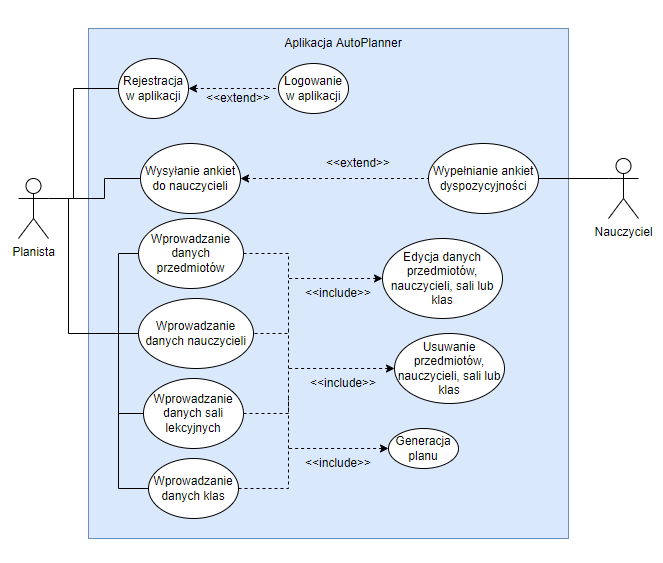
\includegraphics[width=\textwidth]{figures/DiagramPU}
\caption{Diagram przypadków użycia}\label{rys:pu}
\end{figure}


\noindent
\textbf{Przypadek użycia:} Rejestracja w aplikacji\\
\textbf{Aktor główny:} Planista\\
\textbf{Scenariusz główny:}
\begin{enumerate}
	\item Planista wpisuje adres e-mail.
	\item Aplikacja nie zgłasza problemu ze składnią adresu e-mail.
	\item Planista wpisuje nazwę użytkownika oraz hasło.
	\item Planista zatwierdza wprowadzone dane.
	\item Aplikacja akceptuje wprowadzone dane.
	\item Aplikacja tworzy nowe konto użytkownika.
\end{enumerate}
\textbf{Rozszerzenia:}
	\begin{enumerate}
         \item[2.A] Aplikacja zgłasza problem ze składnią adresu e-mail.
         \begin{enumerate}
         	\item[2.A.1] Planista poprawia składnię adresu e-mail.
         \end{enumerate}
         \item[5.A] Aplikacja zgłasza problem  dotyczący wymagań hasła.
         \begin{enumerate}
         	\item[5.A.1] Planista wpisuje hasło, które spełnia wymagania.
         \end{enumerate}
         \item[5.B] Aplikacja zgłasza, że na wpisany adres e-mail jest już założone konto.
         \begin{enumerate}
         	\item[5.B.1] Planista wpisuje nowy adres e-mail.
         \end{enumerate}
	\end{enumerate}
	
\noindent
\textbf{Przypadek użycia:} Logowanie w aplikacji\\
\textbf{Aktor główny:} Planista\\
\textbf{Scenariusz główny:}
\begin{enumerate}
	\item Planista wpisuje adres e-mail.
	\item Planista wpisuje hasło.
	\item Planista zatwierdza wprowadzone dane.
	\item Aplikacja akceptuje wprowadzone dane.
	\item Aplikacja przechodzi do widoku użytkownika zalogowanego.
\end{enumerate}
\textbf{Rozszerzenia:}
	\begin{enumerate}
         \item[4.A] Aplikacja zgłasza, że wprowadzone hasło jest nieprawidłowe.
         \begin{enumerate}
         	\item[4.A.1] Planista ponownie wpisuje hasło.
         \end{enumerate}
         \item[4.B] Aplikacja zgłasza, że użytkownik o podanym adresie e-mail nie istnieje.
         \begin{enumerate}
         	\item[4.B.1] Planista ponownie wpisuje adres e-mail.
         \end{enumerate}
	\end{enumerate}
	
\noindent
\textbf{Przypadek użycia:} Wprowadzanie danych przedmiotów\\
\textbf{Aktor główny:} Planista\\
\textbf{Scenariusz główny:}
\begin{enumerate}
	\item Planista wpisuje nazwę przedmiotu.
	\item Planista zatwierdza wprowadzone dane.
	\item Aplikacja akceptuje wprowadzone dane.
	\item Aplikacja dodaje przedmiot do listy z lewej strony ekranu.
\end{enumerate}
\textbf{Rozszerzenia:}
	\begin{enumerate}
         \item[3.A] Aplikacja zgłasza, że przedmiot o danej nazwie został już wcześniej wprowadzony.
         \begin{enumerate}
         	\item[3.A.1] Planista wpisuje nową nazwę przedmiotu.
         \end{enumerate}
         \item[3.B] Aplikacja zgłasza, że nazwa przedmiotu zawiera niedozwolone znaki.
         \begin{enumerate}
         	\item[3.B.1] Planista wpisuje nową nazwę przedmiotu.
         \end{enumerate}
	\end{enumerate}
	
\noindent
\textbf{Przypadek użycia:} Wprowadzanie danych nauczycieli\\
\textbf{Aktor główny:} Planista\\
\textbf{Scenariusz główny:}
\begin{enumerate}
	\item Planista wpisuje imię i nazwisko nauczyciela.
	\item Planista wpisuje adres e-mail nauczyciela.
	\item Aplikacja nie zgłasza problemu ze składnią adresu e-mail.
	\item Planista wybiera z listy wprowadzony przez nauczyciela przedmiot.
	\item Aplikacja akceptuje wprowadzone dane.
	\item Aplikacja dodaje nauczyciela do listy z lewej strony ekranu.
\end{enumerate}
\textbf{Rozszerzenia:}
	\begin{enumerate}
         \item[3.A] Aplikacja zgłasza problem ze składnią adresu e-mail.
         \begin{enumerate}
         	\item[3.A.1] Planista poprawia składnię adresu e-mail.
         \end{enumerate}
         \item[4.A] Planista dodaje kolejne przedmioty prowadzone przez nauczyciela.
         \item[5.A] Aplikacja zgłasza, że nauczyciel o danym adresie e-mail został już wcześniej wprowadzony.
         \begin{enumerate}
         	\item[5.A.1] Planista wpisuje nowy adres e-mail.
         \end{enumerate}
         \item[5.B] Aplikacja zgłasza, że imię lub nazwisko nauczyciela zawiera niedozwolone znaki.
         \begin{enumerate}
         	\item[5.B.1] Planista wpisuje nowe imię i nazwisko nauczyciela.
         \end{enumerate}
	\end{enumerate}

\noindent
\textbf{Przypadek użycia:} Wprowadzanie danych sal lekcyjnych\\
\textbf{Aktor główny:} Planista\\
\textbf{Scenariusz główny:}
\begin{enumerate}
	\item Planista wpisuje nazwę sali.
	\item Planista nie dodaje preferowanych przedmiotów.
	\item Planista zatwierdza wprowadzone dane.
	\item Aplikacja akceptuje wprowadzone dane.
	\item Aplikacja dodaje salę do listy z lewej strony ekranu.
\end{enumerate}
\textbf{Rozszerzenia:}
	\begin{enumerate}
         \item[2.A] Planista dodaje jeden lub więcej preferowany przedmiot.
         \item[4.A] Aplikacja zgłasza, że sala o danej nazwie została już wcześniej wprowadzona.
         \begin{enumerate}
         	\item[4.A.1] Planista wpisuje nową nazwę sali.
         \end{enumerate}
         \item[4.B] Aplikacja zgłasza, że nazwa sali zawiera niedozwolone znaki.
         \begin{enumerate}
         	\item[4.B.1] Planista wpisuje nową nazwę sali.
         \end{enumerate}
	\end{enumerate}
	
\noindent
\textbf{Przypadek użycia:} Wprowadzanie danych klas\\
\textbf{Aktor główny:} Planista\\
\textbf{Scenariusz główny:}
\begin{enumerate}
	\item Planista wpisuje nazwę klasy.
	\item Planista wybiera z listy kolejne przedmioty.
	\item Planista wpisuje tygodniowe liczby godzin dla każdego przedmiotu.
	\item Planista nie wybiera prowadzącego dany przedmiot.
	\item Planista zatwierdza wprowadzone dane.
	\item Aplikacja akceptuje wprowadzone dane.
	\item Aplikacja dodaje klasę do listy z lewej strony ekranu.
\end{enumerate}
\textbf{Rozszerzenia:}
	\begin{enumerate}
         \item[4.A] Planista wybiera z listy prowadzącego przedmiot.
         \item[6.A] Aplikacja zgłasza, że klasa o danej nazwie została już wcześniej wprowadzona.
         \begin{enumerate}
         	\item[6.A.1] Planista wpisuje nową nazwę klasy.
         \end{enumerate}
         \item[6.B] Aplikacja zgłasza, że nazwa klasy zawiera niedozwolone znaki.
         \begin{enumerate}
         	\item[6.B.1] Planista wpisuje nową nazwę klasy.
         \end{enumerate}
         \item[6.C] Aplikacja zgłasza, że wprowadzona liczba godzin ma nieprawidłowy format.
         \begin{enumerate}
         	\item[6.C.1] Planista wpisuje nową liczbę godzin.
         \end{enumerate}
	\end{enumerate}
	
\noindent
\textbf{Przypadek użycia:} Edycja danych przedmiotów, nauczycieli, sal lub klas\\
\textbf{Aktor główny:} Planista\\
\textbf{Scenariusz główny:}
\begin{enumerate}
	\item Planista wybiera przedmiot, nauczyciela, salę lub klasę, których dane chce edytować.
	\item Aplikacja przechodzi do ekranu edycji z aktualnymi danymi wybranego przedmiotu, nauczyciela, sali lub klasy.
	\item Planista edytuje dane.
	\item Planista zatwierdza edycję danych.
	\item Aplikacja akceptuje edycję danych.
	\item Aplikacja powraca do ekranu dodawania przedmiotu, nauczyciela, sali lub klasy.
\end{enumerate}
\textbf{Rozszerzenia:}
	\begin{enumerate}
         \item[5.A] Aplikacja zgłasza, że nowe dane są nieprawidłowe, w ten sam sposób jak miało to miejsce w przypadku ich dodawania.
         \begin{enumerate}
         	\item[5.A.1] Planista poprawia wpisane dane.
         \end{enumerate}
	\end{enumerate}
	
\noindent
\textbf{Przypadek użycia:} Usuwanie przedmiotów, nauczycieli, sal lub klas\\
\textbf{Aktor główny:} Planista\\
\textbf{Scenariusz główny:}
\begin{enumerate}
	\item Planista wybiera przedmiot, nauczyciela, salę lub klasę, których dane chce edytować.
	\item Aplikacja przechodzi do ekranu edycji z aktualnymi danymi wybranego przedmiotu, nauczyciela, sali lub klasy.
	\item Planista wybiera opcję usuń przedmiot, nauczyciela, salę lub klasę.
	\item Aplikacja usuwa przedmiot, nauczyciela, salę lub klasę z listy z lewej strony ekranu.
\end{enumerate}

\noindent
\textbf{Przypadek użycia:} Wysyłanie ankiet do nauczycieli\\
\textbf{Aktor główny:} Planista\\
\textbf{Scenariusz główny:}
\begin{enumerate}
	\item Planista wybiera opcję 'wyślij ankiety dyspozycyjności' na ekranie dodawania nauczycieli.
	\item Aplikacja wysyła wiadomości e-mail z ankietami dyspozycyjności na adresy e-mail wszystkich do tej pory dodanych nauczycieli.
	\item Aplikacja wyświetla informację, że ankiety zostały wysłane.
\end{enumerate}

\noindent
\textbf{Przypadek użycia:} Wypełnienie ankiety dyspozycyjności\\
\textbf{Aktor główny:} Nauczyciel\\
\textbf{Scenariusz główny:}
\begin{enumerate}
	\item Nauczyciel poprzez link w wiadomości e-mail przechodzi do ekranu wypełniania ankiety.
	\item Nauczyciel zaznacza w siatce godzin swoją dyspozycyjność.
	\item Nauczyciel zatwierdza wprowadzone dane.
	\item Aplikacja zapisuje dane w celu wykorzystania przy generacji planu.
\end{enumerate}

\noindent
\textbf{Przypadek użycia:} Generacja planu\\
\textbf{Aktor główny:} Planista\\
\textbf{Scenariusz główny:}
\begin{enumerate}
	\item Planista wybiera opcję 'generuj plan'.
	\item Aplikacja rozpoczyna generację planu i przechodzi do ekranu oczekiwania.
	\item Aplikacja kończy generację planu i przechodzi do ekranu szkoły.
	\item Planista przegląda wygenerowane plany z podziałem na plany klas, nauczycieli i sal lekcyjnych.
\end{enumerate}